\usetikzlibrary{matrix,backgrounds,positioning,calc,fit}
\definecolor{SceneColor}{RGB}{200,200,200}
\definecolor{GroupColor}{RGB}{90,200,102}
\definecolor{SubGroupColor}{RGB}{114,247,247}

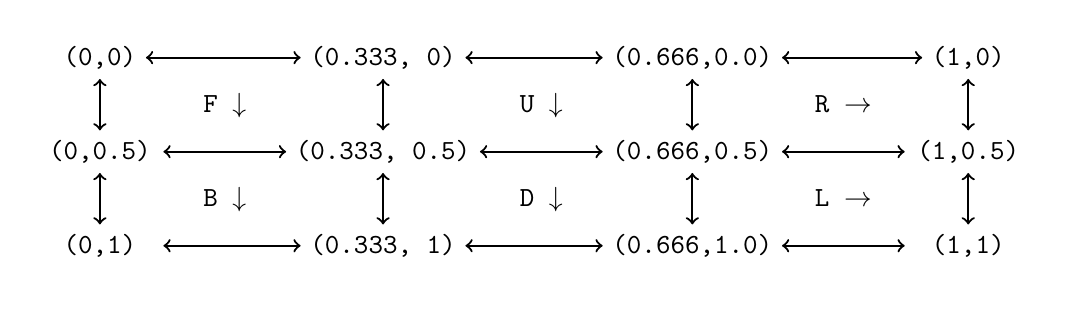
\begin{tikzpicture}[font=\ttfamily,
    array/.style={matrix of nodes,
    nodes={draw=none, minimum width=16mm, minimum height=5mm, fill=white},
    column sep=-\pgflinewidth,
    row sep=-\pgflinewidth,
    nodes in empty cells,
    row 1/.style={nodes={draw=none, fill=none, minimum size=5mm}}}]

    \matrix[array] (Cube) {
        (0,0) &  & (0.333, 0) &  & (0.666,0.0) &  & (1,0) \\
        & F $\downarrow$ &           &  U $\downarrow$ &            & R $\to$ &      \\
        (0,0.5) &  & (0.333, 0.5) &  & (0.666,0.5) &  & (1,0.5) \\
        & B $\downarrow$ &           &  D $\downarrow$ &            & L $\to$ &      \\
        (0,1) &  & (0.333, 1) &  & (0.666,1.0) &  & (1,1) \\
    };

    \foreach \from/\to in {
        Cube-1-1/Cube-1-3, Cube-1-3/Cube-1-5, Cube-1-5/Cube-1-7,
        Cube-3-1/Cube-3-3, Cube-3-3/Cube-3-5, Cube-3-5/Cube-3-7,
        Cube-5-1/Cube-5-3, Cube-5-3/Cube-5-5, Cube-5-5/Cube-5-7,
        Cube-1-1/Cube-3-1, Cube-1-3/Cube-3-3, Cube-1-5/Cube-3-5, Cube-1-7/Cube-3-7,
        Cube-3-1/Cube-5-1, Cube-3-3/Cube-5-3, Cube-3-5/Cube-5-5, Cube-3-7/Cube-5-7}
    \draw [<->, thick] (\from)--(\to);

    % \matrix[array, below = of Scene] (Group2) {
    %     Group 2 \\
    %     Model 4 & Model 5 \\
    %     \\
    % };

    % \matrix[array, left = of Group2] (Group1) {
    %     &  Group 1 & \\
    %     Model 1 & Model 2 & Model 3 \\
    % };

    % \matrix[array, right = of Group2] (Group3) {
    %     Group 3 \\
    %     Model 7 \\
    % };

    % \matrix[array, below = of Group2] (Group21) {
    %     Group 2.1 \\
    %     Model 6 \\
    % };

    % \node[draw, fill=GroupColor, minimum size=2mm, circle] at (Scene-2-1) (Group1Ball) {};
    % \node[draw, fill=GroupColor, minimum size=2mm, circle] at (Scene-2-2) (Group2Ball) {};
    % \node[draw, fill=GroupColor, minimum size=2mm, circle] at (Scene-2-3) (Group3Ball) {};
    % \node[draw, fill=SubGroupColor, minimum size=2mm, circle] at (Group2-3-1) (Group21Ball) {};

    % \begin{scope}[on background layer]
    %     \node[draw, fill=SceneColor, fit = (Scene) (Group1) (Group2) (Group3) (Group21)]
    %     (SceneBox) {};
    %     \node[draw, fill=GroupColor, fit = (Group1)] (Group1Box) {};
    %     \node[draw, fill=GroupColor, fit = (Group2) (Group21)] (Group2Box) {};
    %     \node[draw, fill=GroupColor, fit = (Group3)] (Group3Box) {};
    %     \node[draw, fill=SubGroupColor, fit = (Group21)] (Group21Box) {};
    % \end{scope}

    % \foreach \from/\to in {
    %     Group1Ball/Group1Box, Group2Ball/Group2Box,
    %     Group3Ball/Group3Box, Group21Ball/Group21Box}
    % \draw [->, thick] (\from)--(\to);

\end{tikzpicture}
